\documentclass{article}
\usepackage[utf8]{inputenc}
\usepackage[english, swedish]{babel}

\usepackage{cite}
\usepackage{caption}
\usepackage{graphicx}
\usepackage{float}
\usepackage{textcomp}

\usepackage{listings}
\usepackage{color}
 
\definecolor{codegreen}{rgb}{0,0.6,0}
\definecolor{codegray}{rgb}{0.5,0.5,0.5}
\definecolor{codepurple}{rgb}{0.58,0,0.82}
\definecolor{backcolour}{rgb}{0.95,0.95,0.92}
 
\lstdefinestyle{mystyle}{
    backgroundcolor=\color{backcolour},   
    commentstyle=\color{codegreen},
    keywordstyle=\color{magenta},
    numberstyle=\tiny\color{codegray},
    stringstyle=\color{codepurple},
    basicstyle=\footnotesize,
    breakatwhitespace=false,         
    breaklines=true,                 
    captionpos=b,                    
    keepspaces=true,                 
    numbers=left,                    
    numbersep=5pt,                  
    showspaces=false,                
    showstringspaces=false,
    showtabs=false,                  
    tabsize=2
}

\lstset{style=mystyle}

\usepackage[yyyymmdd]{datetime}
\renewcommand{\dateseparator}{-}

\usepackage{graphicx}
\graphicspath{ {images/} }

%For headers & footers
\usepackage{fancyhdr}
\pagestyle{fancy}
\lhead{
\includegraphics[scale=0.2]{Logo}}
\chead{Kartrobot}
\rhead{\today}

\lfoot{Konstruktion med mikrodatorer}
\rfoot{Grupp 3}

\usepackage{titlesec}

\setcounter{secnumdepth}{4}

\titleformat{\paragraph}
{\normalfont\normalsize\bfseries}{\theparagraph}{1em}{}
\titlespacing*{\paragraph}
{0pt}{3.25ex plus 1ex minus .2ex}{1.5ex plus .2ex}

\renewcommand{\headrulewidth}{0.4pt}
\renewcommand{\footrulewidth}{0.4pt}


\title{Användarhandledning för kartrobot}
\author{Patrik Sletmo}
\date{\today}

\selectlanguage{swedish}

\begin{document}

\thispagestyle{empty}

{
\sffamily
\centering
\large


{\huge 
Användarhandledning för kartrobot
}

{\large
Patrik Sletmo
}

{\large
Version 1.0
}

\vspace{3.5cm}

Status
\begin{table}[H]
\centering
\begin{tabular}{ | c | c | c | }
\hline
Godkänd & Patrik Sletmo & 2016-12-14 \\
\hline
\end{tabular}
\end{table}
}
\clearpage

\vspace*{\fill}
{
\sffamily
\centering
\large


{\huge
Projektidentitet
}

{\large
Grupp 3, 16/HT, KarToffel \\ Linköpings tekniska högskola, ISY
}

\vspace{0.5cm}

\begin{table}[H]
\centering
\begin{tabular}{ | c | c | c | c |}
\hline
Namn & Ansvar & Telefon & E-post \\
\hline
Patrik Sletmo & Projektledare & 070 783 57 61 & patsl736@student.liu.se \\
\hline
Rebecca Lindblom & Utvecklare & 073 436 40 79 & rebli156@student.liu.se \\
\hline
Matildha Sjöstedt & Utvecklare & 070 515 84 11 & matsj696@student.liu.se \\
\hline
Sebastian Callh & Utvecklare & 073 820 46 64 & sebca553@student.liu.se \\
\hline
Anton Dalgren & Utvecklare & 076 836 51 56 & antda685@student.liu.se \\
\hline
Matilda Dahlström & Utvecklare & 070 636 33 52 & matda715@student.liu.se \\
\hline
\end{tabular}
\end{table}
}

\begin{center}
\textbf{Hemsida}: https://github.com/SebastianCallh/kartoffel-tsea29
\end{center}

\begin{center}
\textbf{Kund}: Mattias Krysander, 013 - 28 2198 , matkr@isy.liu.se
\end{center}

\begin{center}
\textbf{Kursansvarig}: Tomas Svensson, 3B 528, +46 (0)13 28 1368, tomas.svensson@liu.se \\
\textbf{Handledare}: Anders Nilsson, 3B 512, +46 (0)13 28 2635, anders.p.nilsson@liu.se
\end{center}
\vspace*{\fill}
\clearpage

\renewcommand*\contentsname{Innehållsförteckning}
\tableofcontents
\clearpage


{
\sffamily
\centering
\large


{\huge 
Dokumenthistorik \\
}
\begin{table}[H]
\centering
\begin{tabular}{ | c | c | c | c | c |} 
\hline
\textbf{Version} & \textbf{Datum} & \textbf{Utförda ändringar} & \textbf{Utförd av } & \textbf{Granskad} \\
\hline
1.0 & 2016-12-14 & Första version & Grupp 3 & Patrik Sletmo \\
\hline

\end{tabular}
\end{table}
}

\clearpage
\section{Inledning}
Det här dokumentet innehåller all information som behövs för att kunna använda roboten KarToffel, en kartrobot skapad av grupp 3 i kursen TSEA29 under höstterminen 2016. Roboten levereras med en mjukvaruklient som används för att både ta emot data från roboten samt styra den manuellt. 


\clearpage
\section{Roboten}
Roboten består av en sedan tidigare byggd robotplattform kallad Terminator med ett antal virkort och komponenter monterade ovanpå. Eftersom roboten inte är byggd med konstruktionssäkerhet i åtanke bör försiktighet vidtagas när den ska förflyttas för att inte råka bryta någon av kopplingarna.

\begin{figure}[H]
\centering
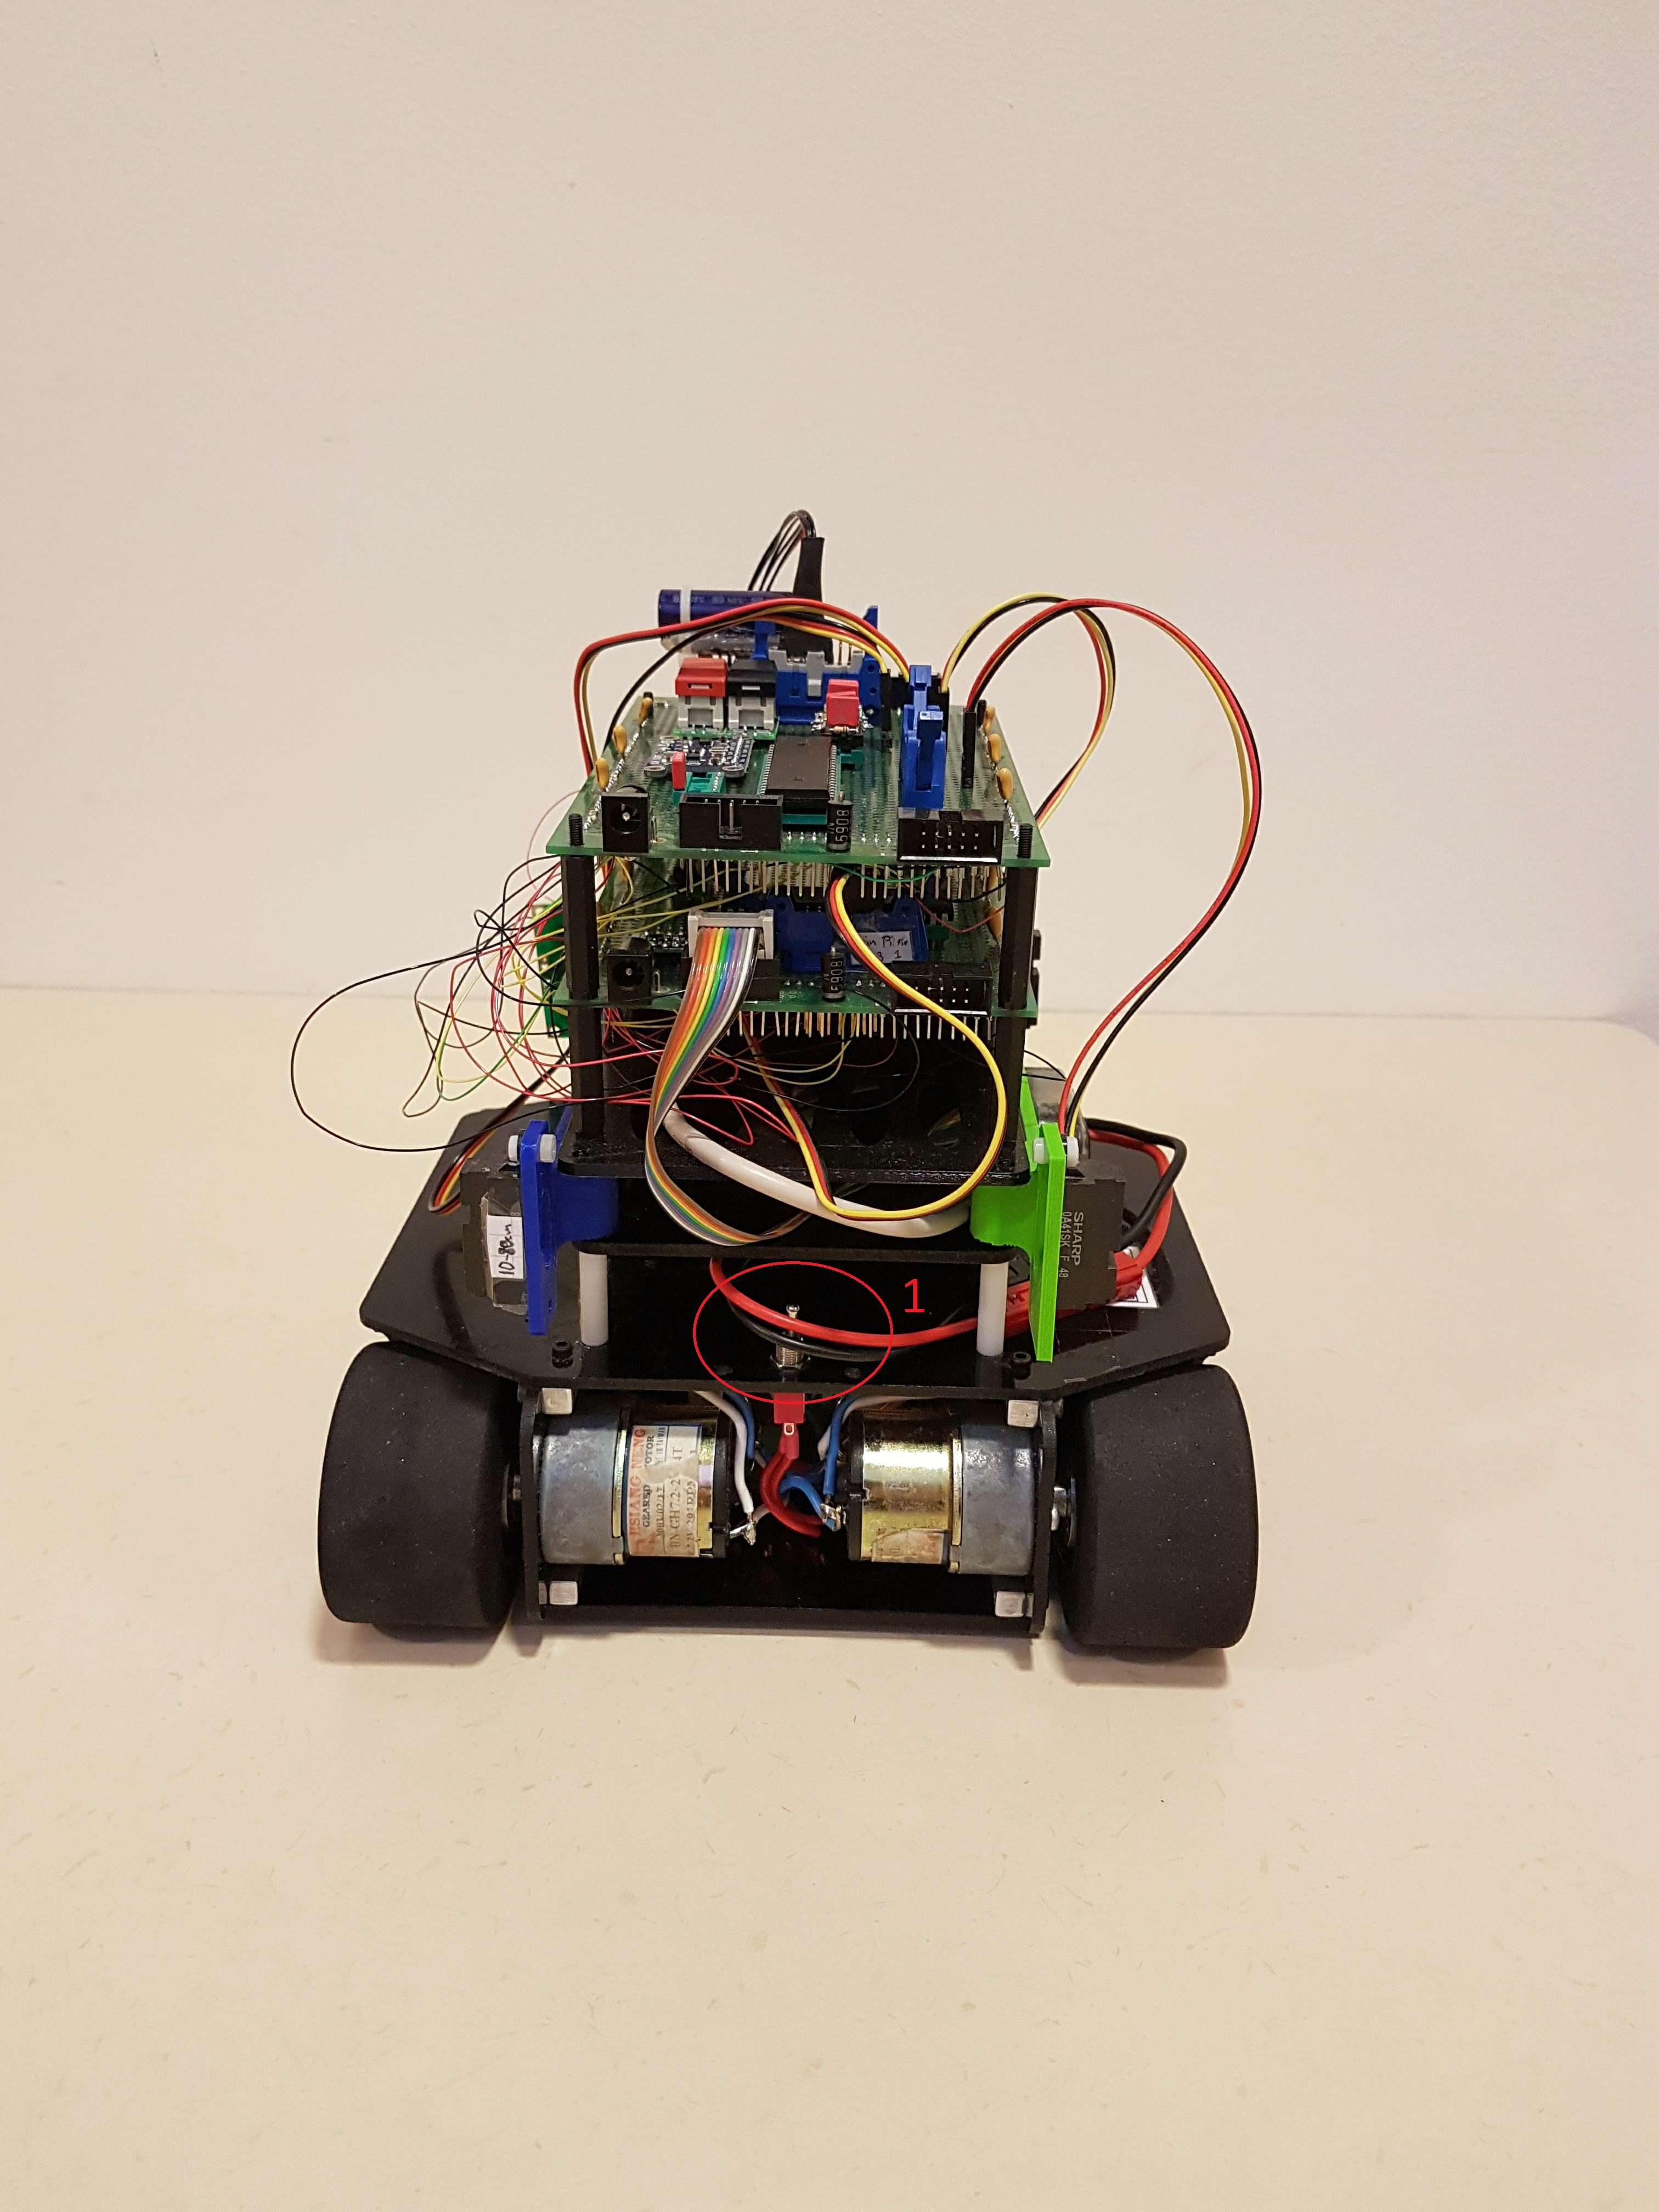
\includegraphics[scale=0.1]{robot_back}
\caption{Roboten sedd bakifrån.}
\label{fig:robot_back}
\end{figure}

\clearpage
\begin{figure}[H]
\centering
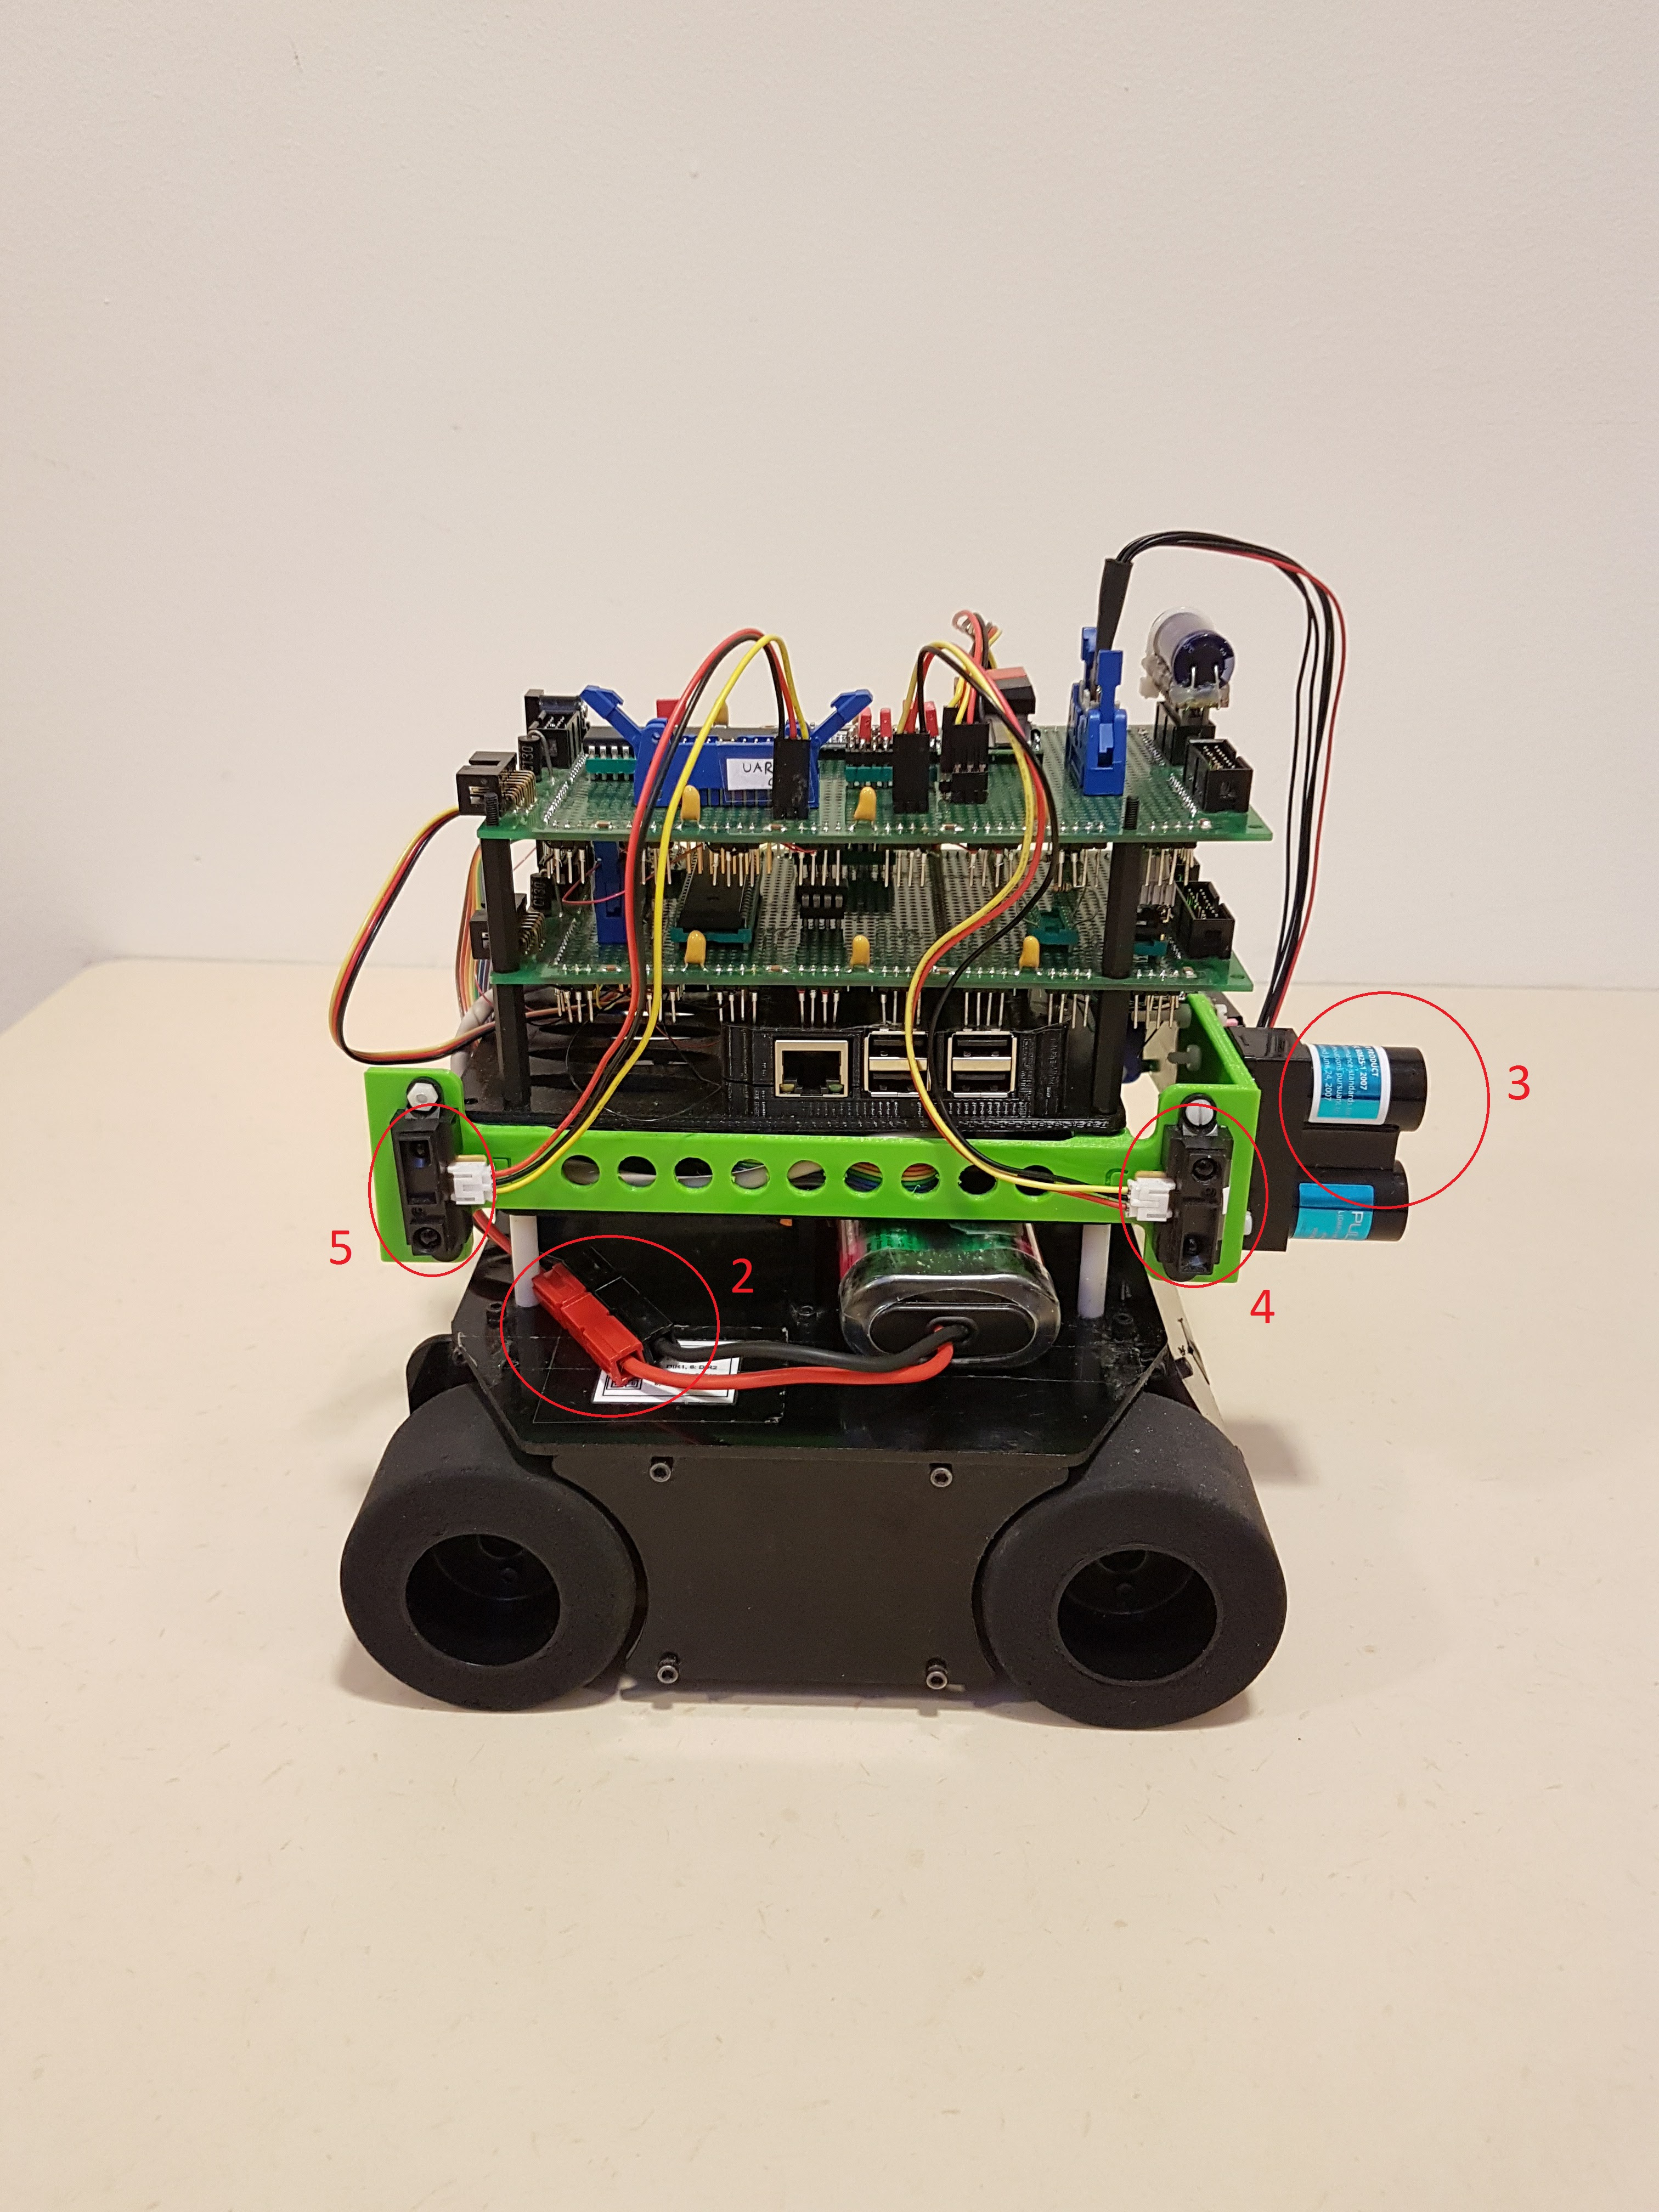
\includegraphics[scale=0.1]{robot_right_side}
\caption{Roboten sedd från höger sida.}
\label{fig:robot_right_side}
\end{figure}

\clearpage
\begin{figure}[H]
\centering
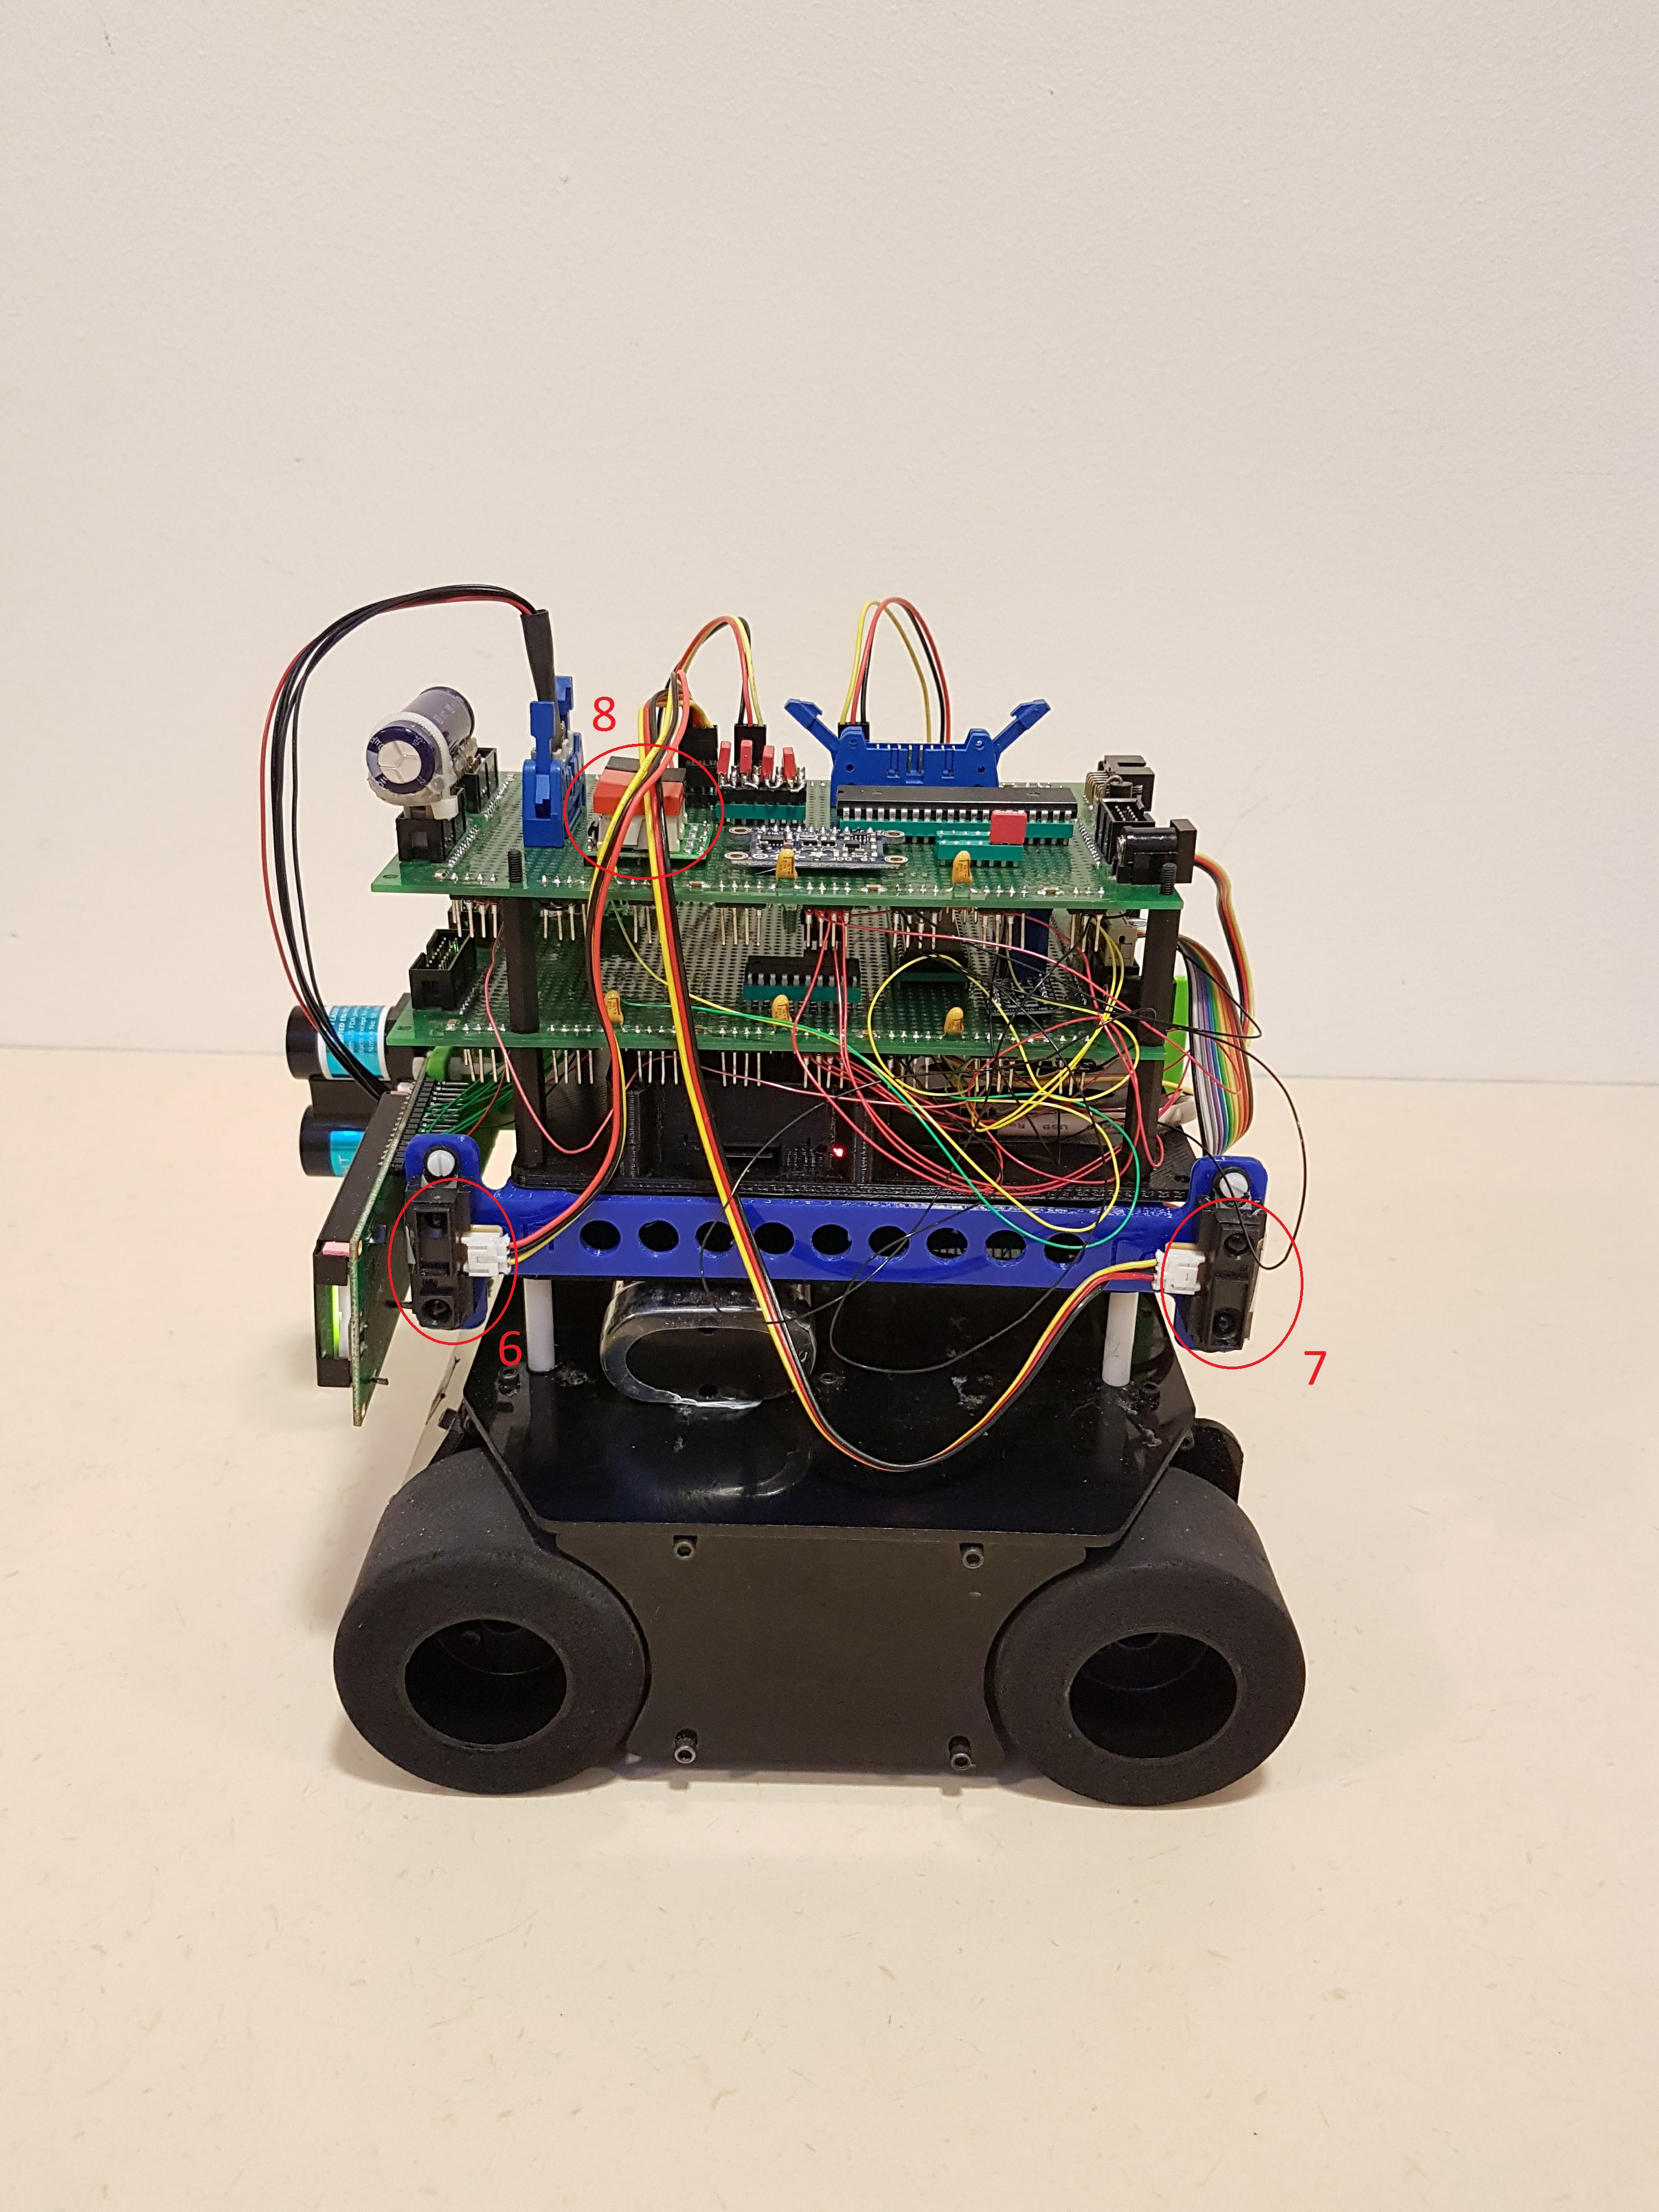
\includegraphics[scale=0.1]{robot_left_side}
\caption{Roboten sedd från vänster sida.}
\label{fig:robot_left_side}
\end{figure}


\begin{table}[H]
\centering
\caption{En tabell över viktiga detaljer på roboten.}
\begin{tabular}{ | c | c | }
\hline
1 & Strömbrytare \\
\hline
2 & Batterianslutning \\
\hline
3 & Lasersensor \\
\hline
4 & Högra främre IR-sensor \\
\hline
5 & Vänstra främre IR-sensor \\
\hline
6 & Högra bakre IR-sensor \\
\hline
7 & Vänstra bakre IR-sensor \\
\hline
8 & Knapp för lägesändring \\
\hline
\end{tabular}
\label{table:components}
\end{table}
\ \\
I figurerna~\ref{fig:robot_back},~\ref{fig:robot_right_side} och~\ref{fig:robot_left_side} syns roboten från olika synvinklar med viktiga detaljer noterade och numrerade enligt tabell~\ref{table:components}. Roboten har två lägen: Ett manuellt läge då den kan styras via mjukvaruklienten, och ett autonomt läge då den själv undersöker ett rum. Trycker man på lägesändringsknappen så byter roboten till det andra läget som den inte är i just då. Roboten startar i manuellt läge. \newline\newline

\clearpage
\section{Mjukvaruklienten}
Till roboten hör en mjukvaruklient skriven i Python som tillhandahåller ett användarvänligt gränssnitt för att skicka indata och ta emot utdata från roboten.

\begin{figure}[H]
\centering
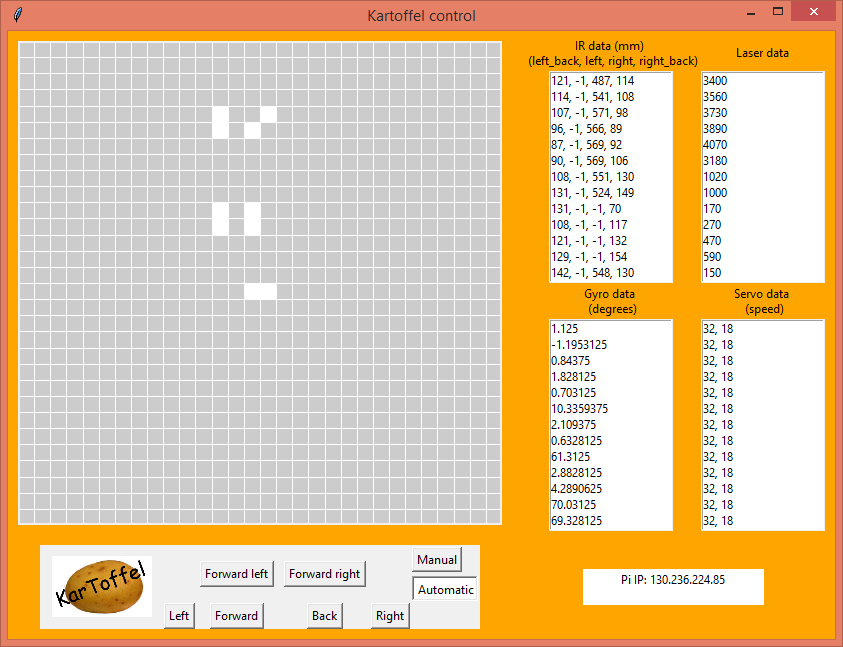
\includegraphics[scale=0.55]{client1}
\caption{Mjukvaruklienten}
\label{fig:client1}
\end{figure}
\ \\
I figur~\ref{fig:client1} visas gränssnittet för mjukvaruklienten. Till höger ses presentation av IR-sensor-, laser-, servo- och gyroskopdata som roboten skickar kontinuerligt oavsett vilket läge den är i. Längst ner till höger syns presentation av robotens IP-adress om den är uppkopplad på ett trådlöst nätverk. 
Till vänster syns det stora området som ritar upp rummet då roboten skickar kartdata. Längst ner till vänster finns knappar för växla mellan manuellt och autonomt läge, samt att styra roboten i det manuella läget. För att styra roboten kan även följande tangenter på tangentbordet användas:
\begin{itemize}
    \item Q - fram vänster
    \item W eller pil upp - framåt
    \item E - fram höger
    \item A eller pil vänster - rotera vänster
    \item S eller pil ner - bakåt
    \item D eller pil höger - rotera höger
\end{itemize}

\clearpage
\section{Installation}
För att ta emot data från roboten samt fjärrstyra den manuellt krävs det att programvaran ``KarToffel Control'' installeras. Programvaran har följande systemkrav:
\begin{itemize}
    \item Operativsystem: Linux eller Windows Vista/7/8/8.1
    \item Python 3 eller senare version
    \item Pybluez, version kompatibel med installerad version av Python
    \item Tkinter, version kompatibel med installerad version av Python
    \item Bluetoothfunktionalitet
\end{itemize}
\ \\
Klienten kräver ingen annan installation än att ladda ner hela katalogen ``client''.

\clearpage
\section{Ansluta till roboten}
Se till att roboten är påslagen med huvudbrytaren och att Bluetooth är aktiverat på datorn. Om det är första gången datorn används för att kopplas upp mot roboten måste datorn paras med roboten via Bluetooth.
\newline\newline
Innan parningen kan genomföras så måste roboten vara upptäckbar över Bluetooth, detta görs genom att exekvera \colorbox{backcolour}{\lstinline{sudo hciconfig hci0 piscan}} i terminalen på roboten. Instruktioner för att ansluta till terminalen finns i dokumentet \textit{Teknisk dokumentation för kartrobot}.
\newline\newline
För att sedan para datorn med roboten används datorns inbyggda gränssnitt för Bluetoothkonfiguration. Där väljs roboten med namn ``raspberrypi'' för anslutning, och inget lösenord anges vid förfrågan. Efter lyckad parning kan mjukvaruklienten startas genom att starta skriptet ``client\textunderscore main.py'' i en lokal terminal. Vid lyckad anslutning till roboten kan knappar och tangenter användas för att kommunicera med roboten. För att avsluta programmet används krysset uppe i högra hörnet för att stänga ner fönstret.

\clearpage
\section{Kommunicera med roboten}
Mjukvaruklienten tar emot data från roboten kontinueligt och presenterar denna data utan att användaren behöver göra något.
Möjliga kommandon för användaren att utföra är att växla mellan manuellt och autonomnt läge samt att styra roboten i det manuella läget. Detta görs med knapparna nere till vänster i gränssnittet.
För att växla mellan manuellt och autonomt läge kan även den fysiska knappen på själva roboten användas. 

\clearpage
\section{Körning i bana}
För att garantera korrekt funktion under bankörning ställs det vissa krav på banans utformande och robotens placering i den. Eftersom roboten är byggd att följa banor som utgår från specifikationen i dokumentet \textit{Ban- och tävlingsspecifikation för kartrobotar 2016} behöver också banor den körs i följa dess begränsningar.
\begin{figure}[H]
\centering
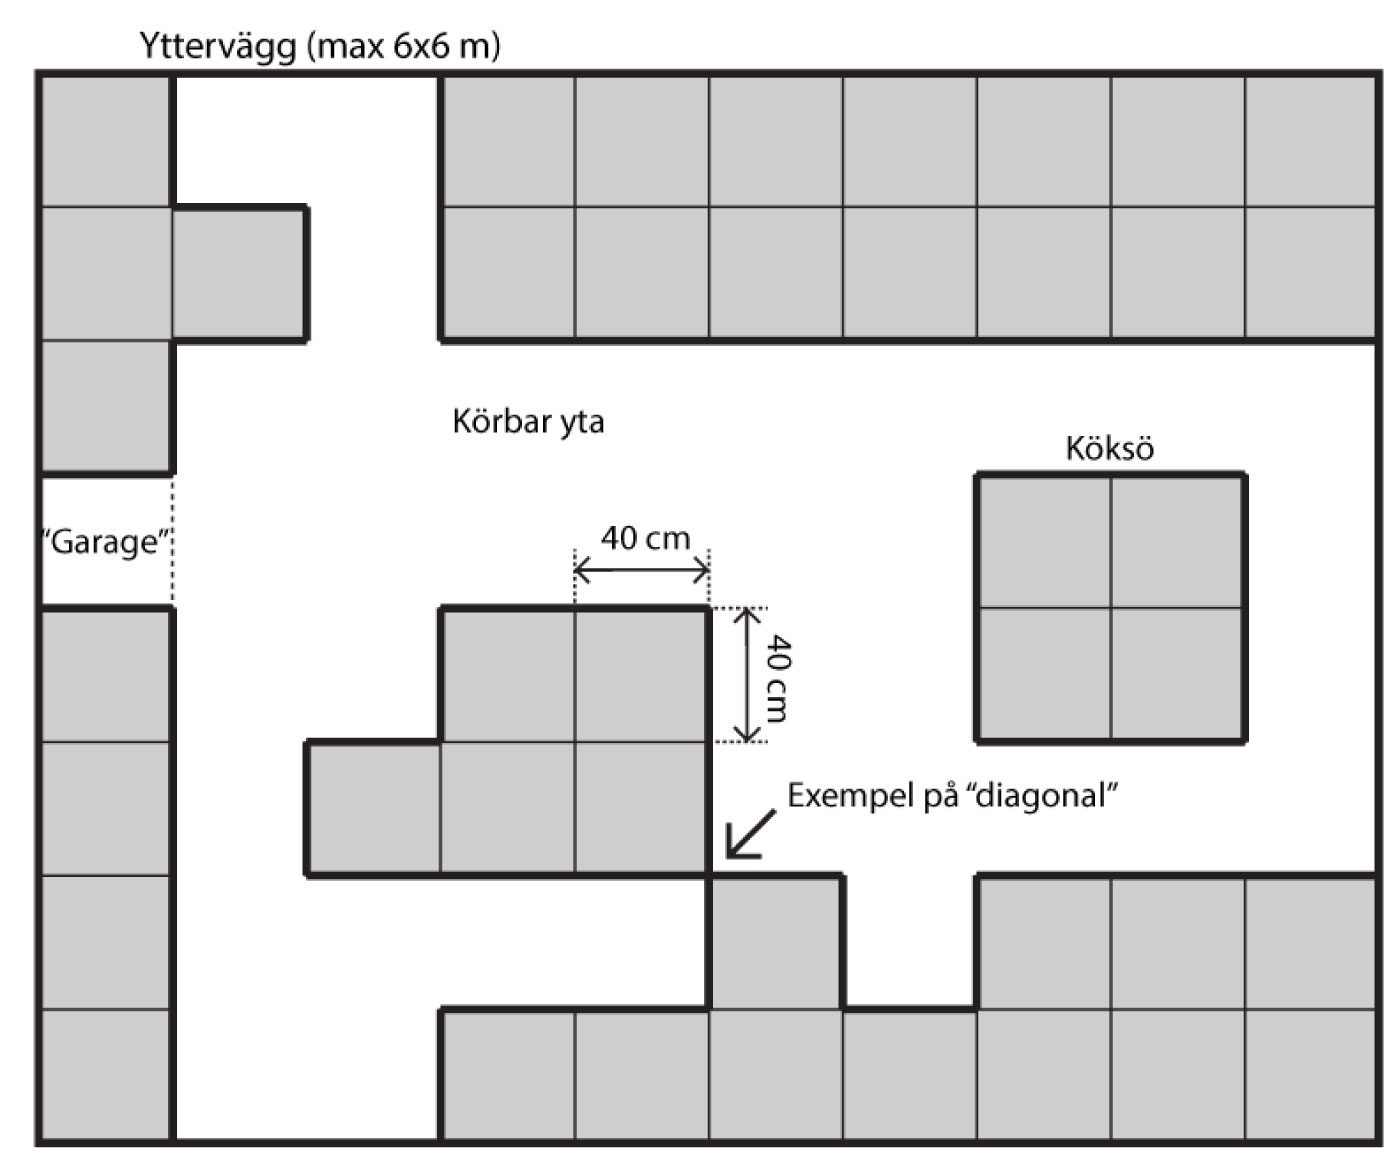
\includegraphics[scale=0.2]{example_map}
\caption{Exempelbana skapad från specifikationen}
\label{fig:example_map}
\end{figure}
\ \\
Roboten behöver även placeras på en speciell punkt i banan för att kunna avsluta kartläggningen korrekt. Innan kartläggningen startar måste roboten placeras i banans så kallade ``garage'' (se figur~\ref{fig:example_map}) och stå med lasern ut från återvändsgränden. När roboten är färdig med kartläggningen återvänder den till detta garage och följer inte garaget specifikationen stannar aldrig roboten.

\clearpage
\section{Referenser}
\begin{itemize}
	\item Pybluez: https://github.com/karulis/pybluez
	\item Tkinter: https://wiki.python.org/moin/TkInter
\end{itemize}

\nocite{*}
\bibliography{designspec}{}
\bibliographystyle{plain}

\end{document}
